\documentclass[a4paper,11pt,twoside,openright]{report}

\usepackage{graphicx}
\usepackage{ngerman}
\usepackage[utf8]{inputenc}
\usepackage{fancyvrb}
\usepackage{courier}
\usepackage{helvet}
\usepackage{tikz}
\usepackage{xcolor}
\usepackage{pdfpages}
\usepackage[strict]{changepage}
\usepackage{float}

\pdfoptionpdfminorversion=6

% \definecolor{se_dark_blue}{RGB}{0,103,166} % powerpoint
\definecolor{se_dark_blue}{RGB}{0,96,178} % website
% \definecolor{se_light_blue}{RGB}{119,158,201} % powerpoint
\definecolor{se_light_blue}{RGB}{129,160,225} % website


%% setup listings
\usepackage{listings}
\lstset{
    numbers=left,
    numberstyle=\tiny,
    numbersep=5pt,
    xleftmargin=11pt,
    xrightmargin=4pt,
    frame=single,
    aboveskip=0pt,
    belowskip=-6pt,
    sensitive=true,
    float=!t,
    breaklines=true,
    captionpos=b,
    tabsize=2,
    showstringspaces=false,
    basicstyle=\small\ttfamily,
    morecomment=[l]{//},
    morecomment=[s][\itshape]{/**}{*/}
}

%% defines the listings laguage named 'MontiArc' derived from the language 'Java'
%% adding the below listed keywords. See
%% ftp://ftp.tex.ac.uk/tex-archive/macros/latex/contrib/listings/listings.pdf
%% for listings documentation
\lstdefinelanguage{MontiArc}[]{Java}{
  morekeywords={component, port, in, out, inv, package, import, connect, autoconnect}
}

% Seite einrichten
\setlength{\voffset}{-1in}
\setlength{\hoffset}{-1in}

\setlength{\topmargin}{2.5cm}
\setlength{\headheight}{0cm}
\setlength{\headsep}{0cm}
\setlength{\oddsidemargin}{3,3cm}  % innen ein wenig mehr Rand für die Klebebindung
\setlength{\evensidemargin}{2,7cm} % dafür außen ein wenig weniger
\setlength{\textwidth}{15cm}
\setlength{\textheight}{23,5cm}
\setlength{\parindent}{0cm}

\newcommand{\emptyLine}{{\LARGE ~\\}}

\begin{document}

% Einrücken von Absätzen verhindern und 1.5 Zeilen Absatzabstand
\setlength{\parindent}{0pt}
\setlength{\parskip}{1.5ex plus0.5ex minus0.5ex}

% Dieses Teildokument beschreibt die Titelseite.
%

% Seitenzähler auf 1, Römische Ziffern.
\setcounter{page}{1}
\pagenumbering{roman}

\thispagestyle{headings}

%\changepage{<text height>}{<text width>}{<even-side margin>}{<odd-side margin>}{<column sep.>}{<topmargin>}{<headheight>}{<headsep>}{<footskip>}
\changepage{5,1cm}{2.4cm}{}{-0.7cm}{}{-2,3cm}{}{}{}

% Eigentliche Titelseite.
\begin{titlepage}
	
\begin{figure}\raggedleft
\includegraphics[height=3.0cm]{src/pic/logo.eps}\end{figure}
  
\begin{tikzpicture}[overlay]

% horizontal lines
\draw[color=se_dark_blue, thick] (-1.6, 0.9) -- (17.4, 0.9);
\draw[color=se_light_blue, thick] (-1.4, 0.7) -- (17.4, 0.7);

% vertical lines
\draw[color=se_dark_blue, thick] (-1, 0.9) -- (-1, -24.5);
\draw[color=se_light_blue, thick] (-0.8, 0.7) -- (-0.8, -24.5);

\end{tikzpicture}

\vspace*{-1.5em}

\begin{flushleft}
  {\fontfamily{phv}  
  	{\LARGE
      Rheinisch Westfälische Technische Hochschule Aachen \\
      Lehrstuhl für Software Engineering \\}
    \vspace{3em}
  
    {\LARGE \textbf{Best Practices of Modern and Efficient Software Engineering}\\} 
    {\LARGE {Anonyme und innere Klassen in Java und ihre Verwendungsmuster}\\} 
    \emptyLine
    \emptyLine 
    \vspace{3em}
		
    {\Large \textbf{Proseminar}\\}
		\vspace{3em} 
		
		{\large von\\} % presented by
    
    {\LARGE \textbf{Birk, Peter 	Jakobi, Felix}\\}
    \vspace{3em} 
		    
    {\Large \textbf{1. Prüfer: Prof.\ Dr.\ B.\ Rumpe}\\}
    \vspace{1em} 
    {\Large \textbf{2. Prüfer: Dipl.-Inform. Deni Raco}\\}
    \vspace{1em} 
    {\Large \textbf{Betreuer: Marlene Lutz}\\}
    \vspace{7em} 

    {\large Diese Arbeit wurde vorgelegt am Lehrstuhl für Software Engineering \\}
    \vspace{1em}
    % The present work was submitted to the chair of software engineering
		{\large	Aachen, den \today\\}
  }
\end{flushleft}

\end{titlepage}

\changepage{-5,1cm}{-2.4cm}{}{0.7cm}{}{2,3cm}{}{}{}





% %Dieses Teildokument beschreibt die Titelseite.
%

% Seitenzähler auf 1, Römische Ziffern.
\setcounter{page}{1}
\pagenumbering{roman}

\thispagestyle{headings}

%\changepage{<text height>}{<text width>}{<even-side margin>}{<odd-side margin>}{<column sep.>}{<topmargin>}{<headheight>}{<headsep>}{<footskip>}
\changepage{5,1cm}{2.4cm}{}{-0.7cm}{}{-2,3cm}{}{}{}

% Eigentliche Titelseite.
\begin{titlepage}
	
\begin{figure}\raggedleft
\includegraphics[height=3.0cm]{src/pic/logo.jpg}\end{figure}
  
\begin{tikzpicture}[overlay]

% horizontal lines
\draw[color=se_dark_blue, thick] (-1.6, 0.9) -- (17.4, 0.9);
\draw[color=se_light_blue, thick] (-1.4, 0.7) -- (17.4, 0.7);

% vertical lines
\draw[color=se_dark_blue, thick] (-1, 0.9) -- (-1, -24.5);
\draw[color=se_light_blue, thick] (-0.8, 0.7) -- (-0.8, -24.5);

\end{tikzpicture}

\vspace*{-1.5em}

\begin{flushleft}
  {\fontfamily{phv}  
  	{\LARGE
      RWTH Aachen University \\
      Software Engineering Group \\}
    \vspace{3em}
  
    {\LARGE \textbf{First line of title}\\} 
    {\LARGE \textbf{Second line of title}\\} 
    {\LARGE \textbf{Third line of title}\\} % Replace with \emptyLine if title is shorter
    {\LARGE \textbf{Forth line of title}\\} % Replace with \emptyLine if title is shorter
    \vspace{3em}
		
    {\Large \textbf{Bachelor Thesis/Master Thesis/Seminar Paper}\\}
		\vspace{3em} 
		
		{\large presented by\\} 
    
    {\LARGE \textbf{Surname, Prename}\\}
    \vspace{3em} 
		    
    {\Large \textbf{1st Examiner: Prof.\ Dr.\ B.\ Rumpe}\\}
    \vspace{1em} 
    {\Large \textbf{2nd Examiner: }\\}
    \vspace{1em} 
    {\Large \textbf{Advisor: }\\}
    \vspace{7em} 

    {\large The present work was submitted to the Chair of Software Engineering \\}
    \vspace{1em}
    % The present work was submitted to the chair of software engineering
		{\large	Aachen, \today\\}
  }
\end{flushleft}

\end{titlepage}

\changepage{-5,1cm}{-2.4cm}{}{0.7cm}{}{2,3cm}{}{}{}




 % English cover

%\clearpage

% Erklaerung

%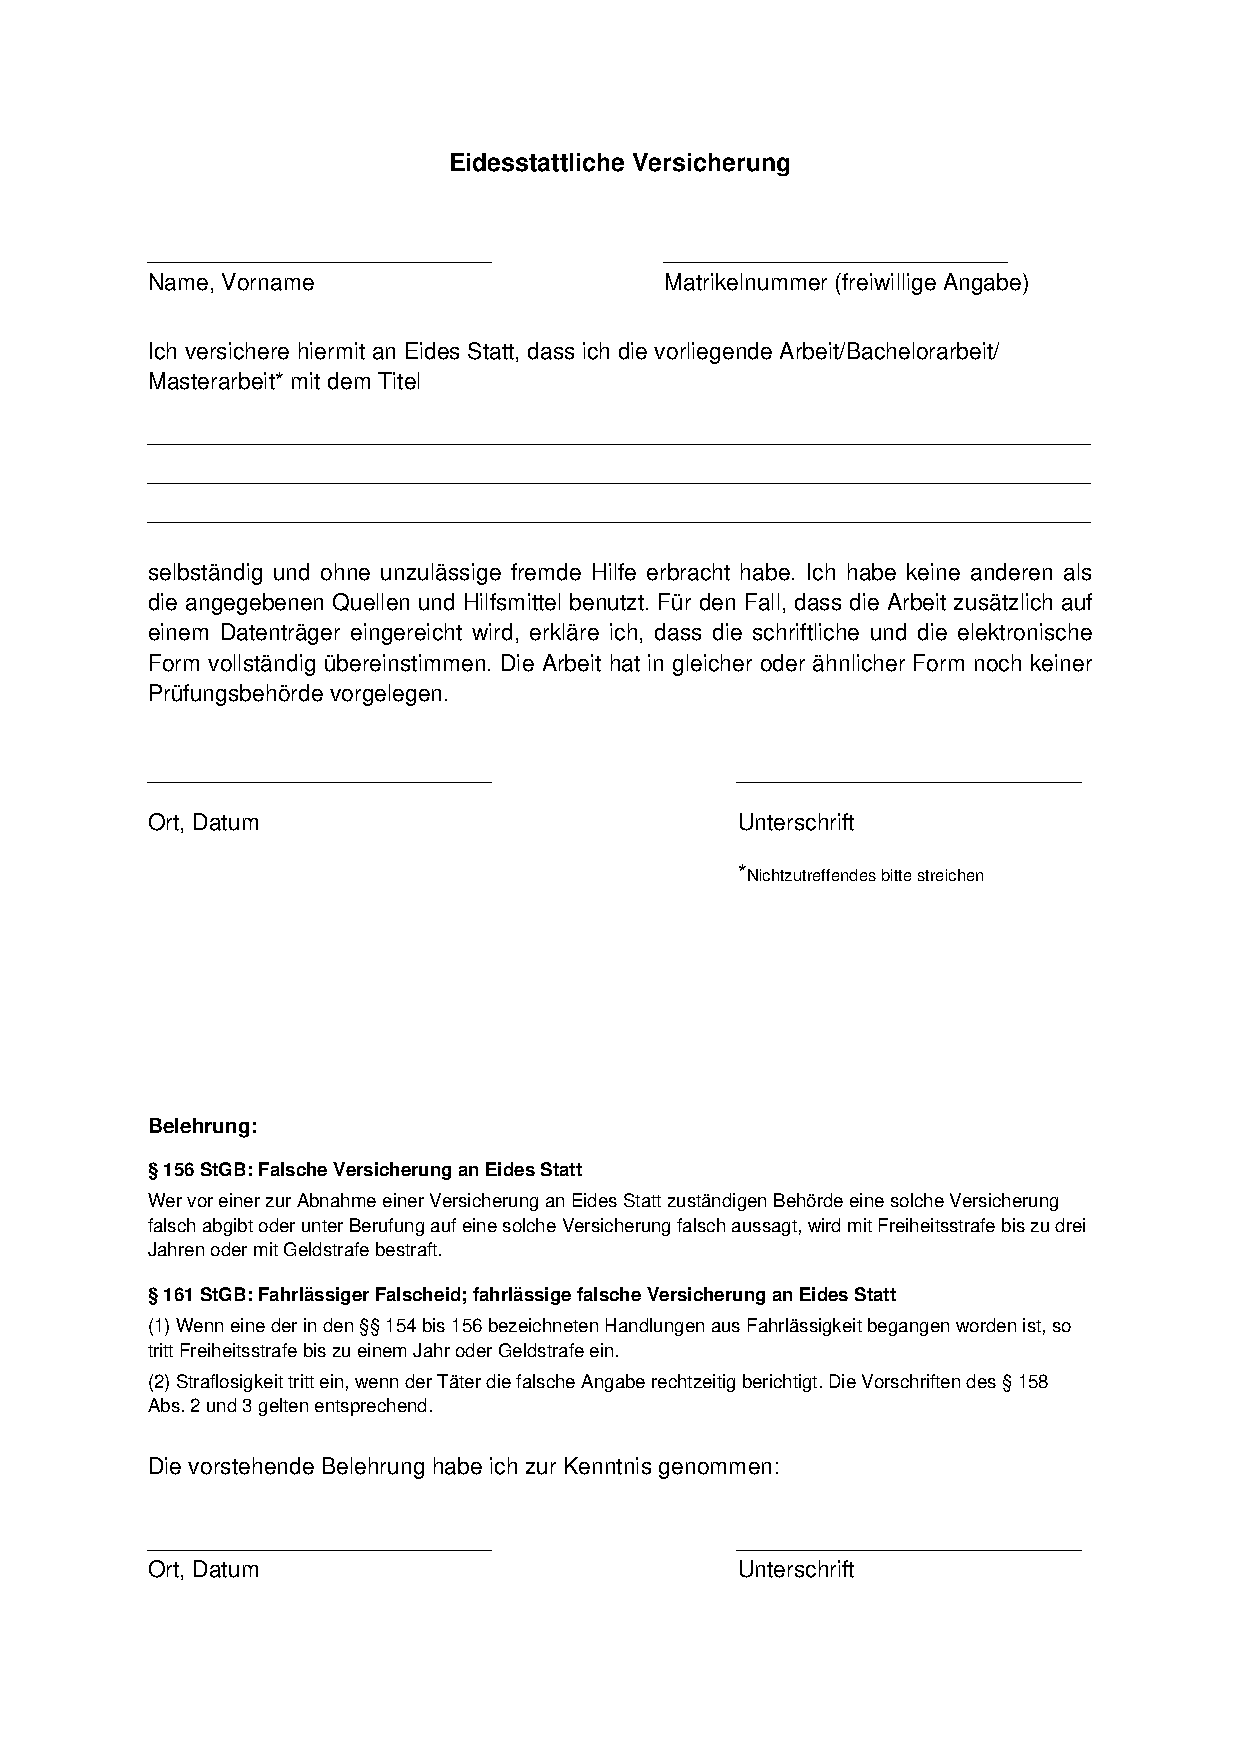
\includepdf[pages={1},offset=-1in -1in]{Formular_Eidesstattliche_Versicherung_neu.pdf}
% 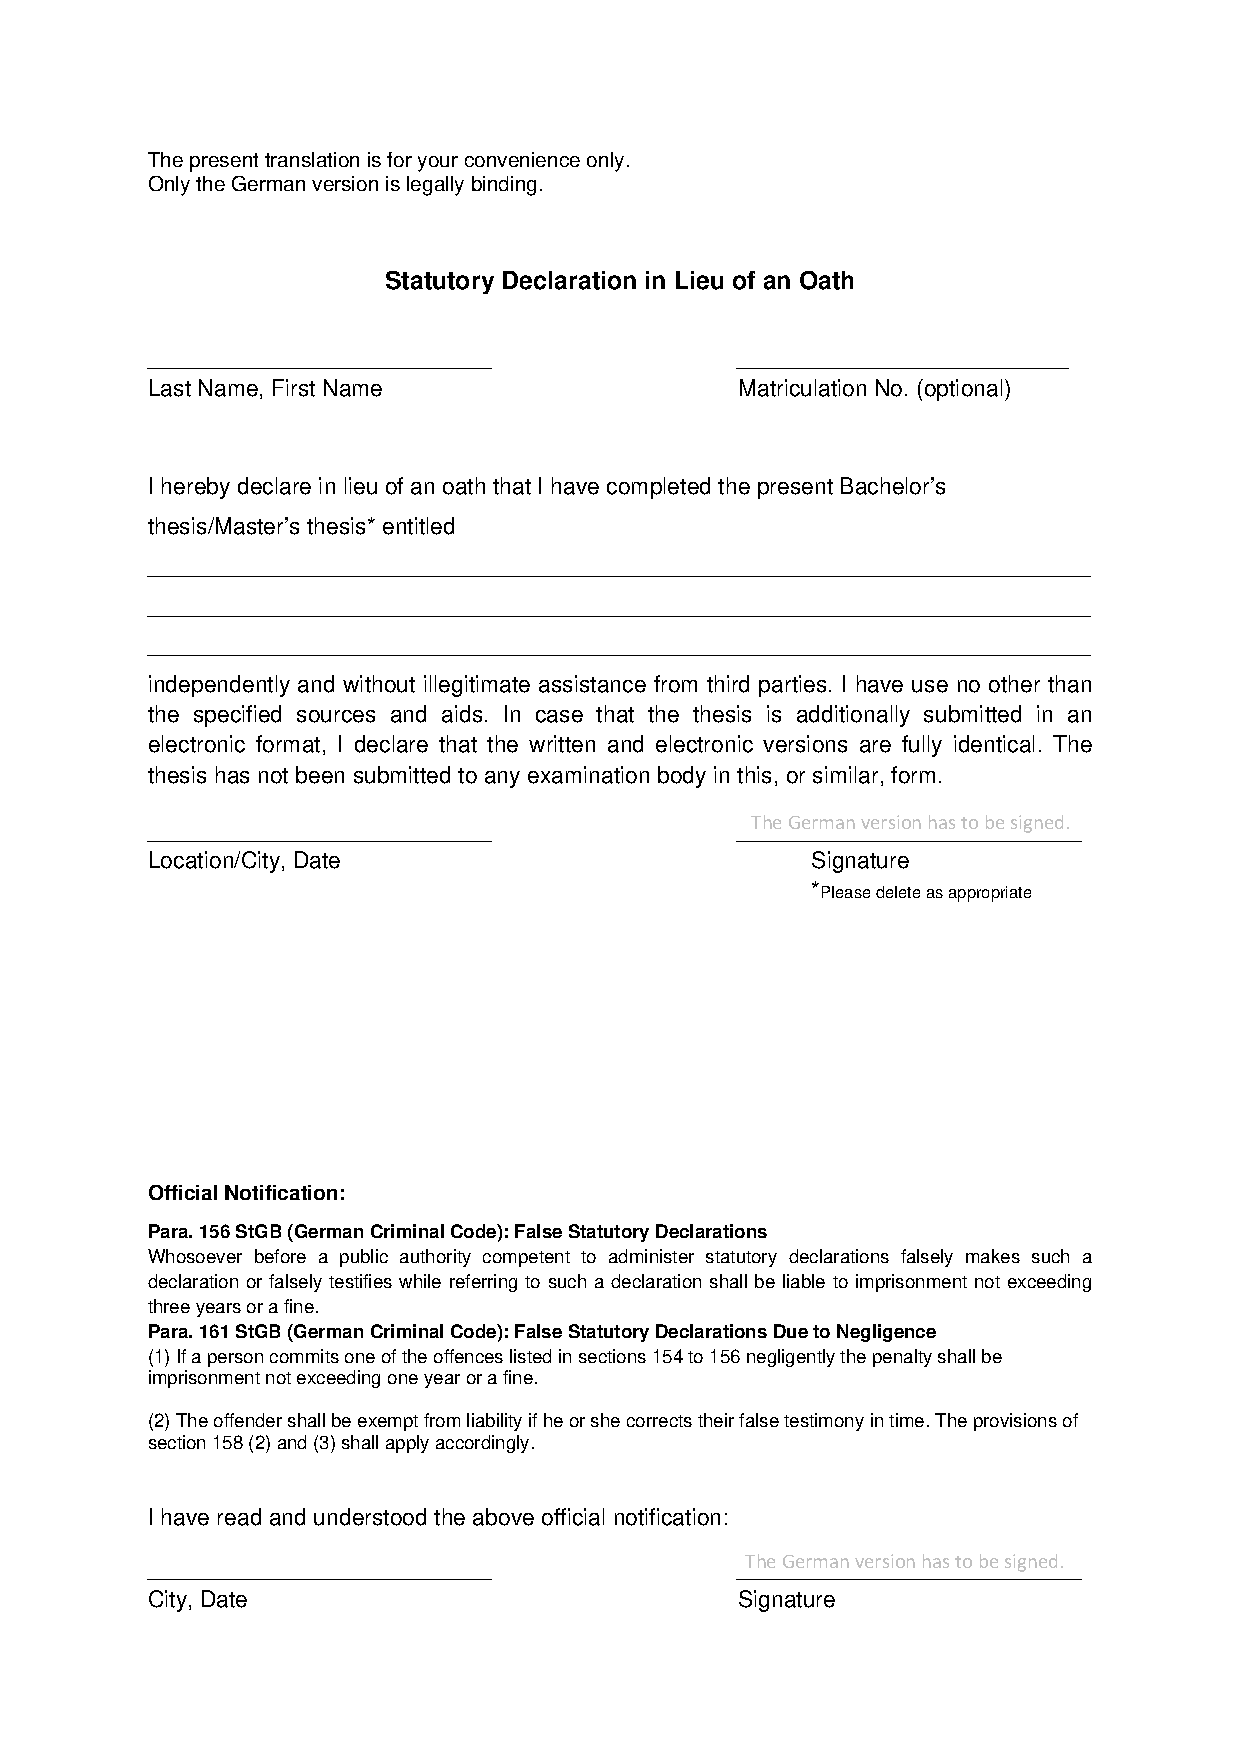
\includepdf[pages={1},offset=-1in -1in]{Statutory_Declaration_in_Lieu_of_an_Oath.pdf} % English

\clearpage

\vspace*{2cm}
% Abstract
{\bf\Large Zusammnefassung} \\ [1em]
Dieses Paper stellt alle gängigen Arten von Eingebetteten Klassen vor.
Nach einer kurzen Einleitung, die einen ersten Überblick ober die verschiedenene Arten gibt, wird ausführlich auf die Implementierung  der verschiedenen Arten eingegangen.
Außerdem werden noch technische Details konkretisiert. Weiterhin werden Vorteile und Nutzen erläutert.
Danach kommt jeweils ein Codebeispiel, in dem eine vorteilhafte Implementierung vorgestellt wird.
Zum Schluss wird noch einmal ein Überblick über das Thema gegeben und der Zusammenhang untereinander und zur konkreten Anwendung hergestellt.
\clearpage


%\vspace*{2cm}
{\Large \textbf{Gliederung:}\\}

	\begin{enumerate}
		\item Einfuehrung
		\begin{enumerate}
			\item Idee/Herkunft
			\item Innere Klassen
			\item Anonyme Klassen
			\item Entwicklung/Geschichte
		\end{enumerate}
	\item Hauptteil
		\begin{enumerate}
			\item (Statische) Innere Klassen
			\begin{enumerate}
				\item Implementierung
				\item Vorteile
				\item Nachteile
				\item Verwendungsmuster
			\end{enumerate}
			\item Anonyme Klassen
			\begin{enumerate}
				\item Implementierung
				\item Vorteile
				\item Nachteile
				\item Verwendungsmuster
			\end{enumerate}
		\end{enumerate}
	\item Zusammenfassung/Fazit
	\item Literaturverzeichnis
	\end{enumerate}
\cleardoublepage


\tableofcontents

\clearpage

% Ab erstem Kapitel Seiten arabisch zählen
\setcounter{page}{1}
\pagenumbering{arabic}

\chapter{Einführung}
\section{Idee / Herkunft}

Innere Klassen wurden in Java 1.1 eingeführt. \cite{Oracle:JDK_Doku1.1.4}
Sie wurden Hauptsächlich eingeführt, da die Java-Designer erkannt hatten, dass die Sprache eine Art "'Funktionszeiger"' benötigt, welcher jedoch mit der Sprachkonstruktion von Java nicht zu realisieren ist.
Diese notwendigkeit kam Haupsächlich von der Existens von Funktionszeigern in anderen Programmiersprachen, wie z.B. C oder Lisp.
Die Möglichkeit, Innere Klassen verschiedenster Art zu benutzen, macht es für die Programmiere einfacher Callbacks und Iteratoren als Adapterklassen zu implemtieren, was vorher umständlich und mit relativ viel aufwand verbunden war.


\clearpage


\chapter{Eingebettete Klassen}
\section{(Statische) Innere Klassen}
\subsection {Implementierung / Instanziierung}

\begin{figure}[H]
\lstset{language=Java}
\lstinputlisting[
label=lst:ImpInn,
escapechar=|,
caption=Beispielimplementierung von inneren Klassen in Java] {src/listings/bsp_ImpInn.java}
\end{figure}

Eine innere Klasse wird in Java durch das Erstellen einer Klasse innerhalb eines bestehenden Klassenblocks implementiert.
Der Name muss unterschiedlich sein. Dabei kann diese mit allen Modifikatoren versehen werden, die auch einer äußeren Klasse zur Verfügung stehen - sie darf aber auch {\it private}, {\it protected} oder {\it static} sein, da sie letzten Endes ein Attribut der äußeren Klasse ist.
Obwohl klassische Mehrfachvererbung (wie in C++) in Java nicht möglich ist, ist es inneren Klassen erlaubt, von einer weiteren Klasse (ausgenommen ihrer äußeren Klasse) zu erben.
Falls es gleichnamige Attribute gibt, wird das Attribut der äußeren Klasse vom Attribut der Oberklasse, von welcher die innere Klasse erbt, verdeckt.
Außerdem können in einer inneren Klasse Attribute implementiert werden. Diese verdecken wiederum gleichnamige Attribute der Ober- oder äußeren Klasse.
Bei einer nicht-statischen inneren Klasse erlaubt Java keine statischen Attribute, da die innere Klasse an sich ein Attribut der äußeren Klasse ist und sonst ein nicht-statisches Attribut statische Elemente enthalten würde.
Falls die Klasse statisch ist, verhält sich diese ähnlich einer normalen Klasse: Es dürfen statische sowie instanzgebundene Attribute verwendet werden, da die Klasse, obwohl sie eigentlich ein statisches Attribut ist, instanziiert werden kann (Listing \ref{lst:ImpInn}).


{\bf Instanziierung}

Eine normale innere Klasse ist an eine Instanz ihrer äußere Klasse gebunden. Bevor der Konstruktor der inneren Klasse aufgerufen werden kann, muss also zuerst eine Instanz der äußeren Klasse generiert werden.
Dann wird der Konstruktor der inneren Klasse von der Instanz der äußeren Klasse aus aufgerufen.
Im Gegensatz dazu benötigt eine statische innere Klasse keine Instanz der äußeren Klasse.
In diesem Fall darf einfach der Konstruktor der statischen inneren Klasse über den Namensraum der Äußeren Klasse aufgerufen werden.
In beiden Fällen werden die Objektdeklarationen über den Namensraum der äußeren Klasse geregelt (Listing \ref{lst:InstInn}) \cite{goll2013java}.

Dies erklärt sich durch Speicherung des Bytecodes der inneren Klassen, welche nach
der Kompilierung als .class Datei im gleichen Ordner wie die äußere Klasse abgelegt
wird. Jedoch wird sie mit {\it ÄußereKlasse\$InnereKlasse.class} bezeichnet, und nicht in der gleichen Datei
gespeichert wie die äußere Klasse.

\begin{figure}[hbt]
\lstset{language=Java}
\lstinputlisting[
label=lst:InstInn,
escapechar=|,
caption=Beispielinstanziierung von inneren Klassen in Java] {src/listings/bsp_InstInn.java}
\end{figure}

{\bf Sichtbarkeit \& Zugriff}

Generell gilt, dass die innere (statische) Klasse je nach Modifikator genau wie ein Attribut der äußeren Klasse gesehen wird, was dann implizit auch für alle Attribute der inneren Klasse gilt, falls diese einer weniger starken Modifikator benutzen.
Auch muss stets der Namensraum der äußeren Klasse benutzt werden, sollte auf Attribute der inneren Klasse zugegriffen werden.
Weiterhin hat die innere Klasse im Normalfall Zugang zu allen Methoden und Variablen der äußeren Klasse - sogar zu denen, die als private deklariert wurden.
Dies gilt andersherum ebenso: Auch die äußere Klasse kann auf die komplette innere Klasse zugreifen, gleich ob diese privat ist oder nicht.
Eine große Unterscheidung muss jedoch gemacht werden wenn eine innere Klasse statisch ist. Da in diesem Fall keine Instanz der äußeren Klasse verbunden ist, können auch lediglich statische Attribute der äußeren Klasse benutzt werden (Listing \ref{lst:SZInn}).
\\
\\
\begin{figure}[hbt]
\lstset{language=Java}
\lstinputlisting[
label=lst:SZInn,
caption=Sichtbarkeitsbeispiel für innere Klassen in Java] {src/listings/bsp_SZ_Inn.java}
\end{figure}

\subsection{Vorteile und Nutzen}

Ein Grund für die Benutzung der inneren Klassen ist die Möglichkeit, innerhalb der inneren Klasse auf die privaten Attribute der äußeren Klasse zugreifen und modifizieren zu können.
Dies ist insbesonders ein Vorteil für die Datenkapselung, da man innerhalb der inneren Klasse mithilfe von Funktionen der Oberklasse alle Attribute der äußeren Klasse bearbeiten kann, ohne dass die Oberklasse (und somit weitere Klassen) Zugriff auf diese Daten haben können.

Ein Grund dafür ist die Möglichkeit, dass eine innere Klasse, welche implizit die Methoden und Variablen der äußeren Klasse erbt, eine weitere Oberklasse erweitern kann und somit auch deren Variablen und Methoden erbt.
Außerdem können Klassen, welche von der inneren Klasse erben (was möglich ist, wenn diese nicht als private, protected oder final markiert sind) über die innere Klasse auf die Attribute und Methoden der äußeren Klasse zugreifen, ohne dass diese direkt von ihr erbt. Dies kann jedoch auch zu Problemen führen.

Es entsteht dadurch die Möglichkeit, dass es durch die Sichtbarkeit der inneren Klasse nach außen zu zyklischen Vererbungen kommt. Dies bedeutet, dass eine Klasse (indirekt) von sich selbst erbt und somit eventuell eigene Methoden überschreibt (\cite{DBLP:journals/corr/abs-1301-6260}) (Listing \ref{lst:ZclInn}).
Im Beispiel \ref{lst:ZclInn}  wird die zyklische Vererbung nicht erkannt, da die Klasse {\it innerA} die Klasse {\it A} nicht erweitert und somit nicht direkt von ihr erbt. Damit kann der Java-Compiler die Tatsache, dass {\it innerA} durch {\it A} von {\it B} erbt, nicht erkennen, und der Code wird fehlerlos kompliiert.
Dies kann, wenn es nicht bemerkt wird, zu falschem, und aus der Sicht der Entwickler, sonderbarem Verhalten führen, obwohl die Implementierung semantisch korrekt ist.
Um die Möglichkeit zu verringern, dass eine zyklische Vererbung auftreten kann, wurde das sogenannte PICIP (Eine Kurzform für "'Potential Inner Class Inheritance Problem"') enwickelt, welches das Potential beschreibt, mit dem Vererbungsprobleme bei inneren Klassen auftreten könnten.
\\
\\
\begin{figure}[hbt]
\lstset{language=Java}
\lstinputlisting[
label=lst:ZclInn,
escapechar=|,
caption=Von Java nicht erkannte Zyklische Vererbung] {src/listings/bsp_Zcl_A.java}
\end{figure}

Weiterhin wird durch Einsatz innerer Klassen die Implementierung einer Adapterklasse erleichtert, welche genau an der Stelle mit den entsprechenden Methoden einer externen Klasse deklariert werden kann.

Man kann durch die Deklaration einer benötigten Klasse als innere Klasse an der entsprechenden Stelle die Lesbarkeit/Übersichtlichkeit des Codes erhöhen.
Dadurch ist es jedoch auch möglich, dass der Code durch zu viele bzw. zu tief ineinander verschachtelte innere Klassen unübersichlich und somit unangenehm zu lesen wird.
Allgemein gilt daher, dass so wenig innere Klassen wie möglich ineinander geschachtelt werden sollten, um besonders die Fehlererkennung zu verbessern.

Außerdem werden Namenskonflikte mit anderen Klassen im Paket vermieden, da man mehrere Klassen mit gleichem Namen haben kann,
die (statischen) inneren Klassen jedoch über ihre äußere Klasse instanziiert werden müssen und es somit nicht zu Verwechslungen und Konflikten mit gleichnamigen Klassen im Paket kommen kann.

\subsection{Anwendungen / Best Practices}

Innere Klassen sollten hauptsächlich dann verwendet werden, wenn eine Klasse ausschließlich von der Oberklasse benutzt wird.
Ein weiterer Anwendungsfall wäre die Ausnutzung der Mehrfachvererbung oder die Möglichkeit, neuen Methoden Zugriff auf die privaten Attribute der äußeren Klasse zu erlauben.

{\bf Beispiel \ref{lst:AnwInn}: Der Ladeadapter}

In diesem simplen Beispiel geht es darum, einen Adapter für den Ladevorgang eines Handys der Marke A zu bauen. Dabei benutzen wir eine Adapterklasse, welche ein Strukturmuster aus der Softwaretechnik ist. Wenn eine Klasse Methoden einer anderen Klasse benötigt, jedoch nur ein Objekt hat, welches ein Interface implementiert, so kann man eine Adapterklasse benutzen.
Wir benötigen für das HandyA ein Objekt, welches das Interface {\it Ladegeraet} implementiert.
Wir haben jedoch kein passendes Ladegeraet von A zur Verfuegung, sondern nur ein Ladegeraet einer Marke B, welches das Interface nicht implementiert.
Da jedoch auch dieses im Prinzip laden kann, versuchen wir, diese Funktionalität für unser Handy zu benutzen.
Dies können wir durch die Einbindung der innere Klasse Adapter erreichen, welche das Interface implementiert.
Jedoch steht uns hier auch das Ladegeraet der Marke B zur Verfügung.
Dieses instanziieren wir und überschreiben die Methode des Interfaces dadurch, dass wir hier die Lademethode des Handy B benutzen.
Damit können wir eine Instanz des Adapters als Ladegeraet für unser Handy benutzen, obwohl uns kein "'korrektes"' Ladegeraet zur Verfügung stand.
\\
\begin{figure}[hb]
\lstset{language=Java}
\lstinputlisting[
label=lst:AnwInn,
escapechar=|,
caption=Beispielanwendung von inneren Klassen in einem Adapter] {src/listings/bsp_AnwInn.java}
\end{figure}


\newpage


\section{Anonyme \& Lokale Klassen}
\subsection {Implementierung}

{\Large \bf Anonyme Klassen}

Eine anonyme Klasse wird in Java nach Konstruktoraufruf einer beliebigen Klasse / Interfaces definiert (Listing \ref{lst:ImAnn}).
Dazu wird nach dem Aufruf ein Codeblock mit geschweiften Klammern geöffnet, in dem die instanziierte Klasse beliebig um Methoden und Datenfelder erweitert werden kann, welche nicht statisch sein dürfen.
Da die Anonyme Klasse von der eigentlich instaziierten Klasse erbt und somit eine Unterklasse dieser ist, können dabei auch Methoden überschrieben werden.
Die konkrete Instanz kann jedoch selbst nur auf schon in der Oberklasse deklarierte Methoden und Variablen zugreifen, da das Objekt der Anonymen Klasse automatisch zu einem Objekt der Oberklasse gecastet wird, welche jedoch selbst, wenn sie überschrieben werden, auch auf die Methoden der Anonymen Klasse Zugreifen dürfen.
Da diese eigentlich neue Klasse keinen Namen zugewiesen bekommen hat, wird sie anonym genannt.
Aufgrund des einmaligen, instanzgebundenen Auftretens einer anonymen Klasse sind weitere Modifikatoren weder sinnvoll noch möglich (\cite{goll2013java}) (\cite{Oracle:JLS9}).

\begin{figure}[h]
\lstset{language=Java}
\lstinputlisting[
label=lst:ImAnn,
escapechar=|,
caption=Beispielimplementierung und -instanziierung einer Anonymen Klasse in Java] {src/listings/bsp_ImAnn.java}
\end{figure}

{\bf Sichtbarkeit \& Zugriff}

Es liegt in der Natur der Anonymen Klassen, dass auf sie lediglich über die mit ihr verbundenen Instanz zugegriffen werden kann.
Weiterhin kann die anonyme Klasse auch nur mit ihren eigenen Attributen bzw. denen der Oberklasse arbeiten.

\newpage

{\Large \bf Lokale Klassen}

{\bf Implementierung}

Lokale Klassen sind Innere Klassen, welche in Methoden eingebunden werden (Listing \ref{lst:ImLok}).
Im Gegensatz zu den Inneren Klassen können hier keine zusätzliche Modifiers verwendet werden, da die lokale Klasse nicht das Attribut einer Klasse ist.
Weiterhin darf sie nicht den Namen der umschließenden Klasse haben.
Die lokale Klasse darf jedoch von einer anderen Klasse erben und nicht-statische Attribute haben.

{\bf Sichtbarkeit und Zugriff}

Die lokale Klasse an sich ist nur innerhalb der Methode sichtbar. Welche Art von Zugang die lokale Klasse zur umschließenden Klasse hat, hängt vom Modifier der einschließenden Methode ab, verläuft aber sonst parallel zu den inneren Klassen.
Ist die Methode statisch, kann die lokale Klasse somit auch nur auf statische Attribute der umschließenden Klasse zugreifen. Ist die Methode wiederum instanzgebunden, dann hat diese auf alle Attribute der umschließenden Klasse Zugriff.
Auf Methodenvariablen selbst hat die Klasse keinen Zugriff, außer diese wurden als final deklariert. Falls die lokale Klasse erbt, verdecken gleichnamige Attribute der Oberklasse die der umschließenden Klasse.
\\
\\
\begin{figure}[ht]
\lstset{language=Java}
\lstinputlisting[
label=lst:ImLok,
escapechar=|,
caption=Beispielimplementierung einer Lokalen Klasse in Java] {src/listings/bsp_ImLok.java}
\end{figure}

\newpage
\newpage

\subsection{Vorteile / Nutzen}

{\bf Anonyme Klassen}

Anonyme Klassen werden haupsächlich und im Idealfall nur benutzt, wenn man eine modifizierte Instanz einer Klasse bzw. eine Instanz eines Interfaces nur einmal gebraucht wird und somit das übertragen der Modifikationen in eine (Innere) Klasse nicht sinnvoll wäre.
Außerdem werden sie benutzt um Instanzen von Abstrakten Klassen zu erzeugen, da man direkt die abstrakten Methoden überschreiben kann, ohne vorher eine neue Unterklasse der entsprechenden Abstrakten Klasse zu deklarieren.
Somit hilft die Benutzung von Anonymen Klassen der Übersichtlichkeit, Lesbarkeit und Verständnis des Codes, da Veränderungen an den Klassen direkt an den benötigten Stellen durchgeführt werden.
Wenn die Modifikationen jedoch in verschiedenen Klassen bzw. Methoden gebraucht werden, sollte jedoch auf eine (Statische) Innere Klasse ausgewichen werden, um die Lesbarkeit des Codes zu erhöhen.

{\bf Lokale Klassen}

Die Lokale Klasse kann nur im Bereich ihrer Methode eingesetzt werden und nicht als Oberklasse dienen.
Lokale Klassen sollten nur benutzt werden, wenn die neu implementierten Methoden nur in der entsprechenden Methode gebraucht werden.
Wenn diese Funktionen jedoch möglicherweise in mehreren Methoden der Äußeren Klasse benötigt werden, sollte jedoch eine Innere Klasse bzw. "'Normale"' Klasse benutzt werden.

\newpage
\subsection{Anwendung / Best Practices}


\begin{figure}[H]
\lstset{language=Java}
\lstinputlisting[
label=lst:AnwAnn,
escapechar=|,
caption=Mögliche GUI-Implementierung mit Inneren Klassen] {src/listings/bsp_AnwAnn.java}
\end{figure}


{\bf Beispiel: Eine einfache GUI mit Inneren / Anonyme Klassen}

In diesem einfachen Anwendungsbeispiel soll die Anwendung in einem Graphical User Interface (GUI) modelliert werden, die ereignisgesteuert ist.
Es gibt zwei Buttons, die nach Drücken etwas tun sollen.
Die Ereignisbehandlung an sich wird hierbei durch Elemente des Windows Abstract Toolkit (aus jawa.awt) geregelt.
Um nun die Ereignisbehandlung zu implementieren, brauchen wir eine Klasse, welche das ActionListener-Interface aus dem Toolkit implementiert und die Methode dem Aufrufer entsprechend ändert.
Insgesamt benötigen wir also 3 Klassen: Die Anwendung (ButtonPressing), die GUI (GUI) und die Ereignisbehandlung (MyEventHandler). Dabei wird die Ereignisbehandlung nur von der GUI benutzt, die GUI wiederum nur von der Anwendung. Dabei benutzt die Ereignisbehandlung Methoden, die in der Anwendung aufgerufen werden müssen.
Die Klassen sind also semantisch stark miteinander verbunden und brauchen teilweise vollen Zugriff aufeinander.
Aus den Umständen folgt, dass hier eine entsprechende Schachtelung der Klassen von Vorteil wäre, was sich sehr gut mit den inneren Klassen realisieren lässt.
Dabei wird die Ereignisbehandlung eine innere Klasse des GUI, die ihrerseits eine innere Klasse der Anwendung wird (Listing \ref{lst:AnwAnn}).
So lässt sich der Code prägnant an der Stelle formulieren, wo er gebraucht wird.
Währenddessen sind die betroffenen Klassen sonst komplett unsichtbar.
Doch hier können auch die anonymen Klassen genutzt werden, denn momentan agiert nur eine Instanz des EventHandlers, die je nach Button einen Unterschied macht. Es kann jedoch deutlich eleganter sein, mehrere "'Einweginstanzen"' zu haben, die dann nur auf einen Button reagieren und dementsprechend nur eine Methode überschreiben müssen.
Dadurch fällt der Overhead durch if-Cases weg und man kann noch klarer sehen, was durch das Drücken eines bestimmten Buttons ausgelöst werden soll (Listing \ref{lst:AnwAnnB}).
\\
\begin{figure}[H]
\lstset{language=Java}
\lstinputlisting[
label=lst:AnwAnnB,
escapechar=|,
caption=Mögliche GUI-Implementierung mit Anonymen statt Inneren Klassen] {src/listings/bsp_AnwAnnB.java}
\end{figure}
\newpage
{\bf Beispiel für lokale Klassen: Kuchenverkostung}

In diesem Beispiel soll das Essen eines Kuchens modelliert werden.
 Dabei gibt es die Klasse Kuchen. Der Kuchen kann je nach seinem Geschmack Feedback bekommen.
Dieses Feedback kommt von verschiedenen Menschen, die unterschiedliche Geschmäcker haben.
Da die Kuchentester jedoch nur in dieser Methode gebraucht werden, implementieren wir sie auch nur in einer lokalen Klasse in getFeedback.
\\
\begin{figure}[H]
\lstset{language=Java}
\lstinputlisting[
label=lst:AnwLok,
escapechar=|,
caption=Beispiel für die Anwendung von lokalen Klassen] {src/listings/bsp_AnwLok.java}
\end{figure}


\chapter{Zusammenfassung und Ausblick}

% Bild einbinden
\begin{figure}[ht!]
\begin{center}
\includegraphics[width=5cm]{src/pic/logo}\end{center}
\caption{Das SE Logo}
\label{Logo}
\end{figure}

\cleardoublepage


\bibliographystyle{alpha}
\addcontentsline{toc}{chapter}{Literaturverzeichnis}
\bibliography{src/bib/Literatur.bib}

% Begin Anhang
%\appendix
%\chapter{z.\,B. Programmdokumentation}

\cleardoublepage


\end{document}
